\documentclass[aspectratio=169,11pt]{beamer}

\usepackage[T1]{fontenc}
\usepackage[english]{babel}
\usepackage{lmodern}
\usepackage{booktabs}
\usepackage{array}
\usepackage{graphicx}
\usepackage{xcolor}
\usepackage{hyperref}

\graphicspath{{assets/}}

% agent-mem UI palette
\definecolor{amBg}{HTML}{0D0F10}
\definecolor{amPanel}{HTML}{111516}
\definecolor{amPanelTwo}{HTML}{15191A}
\definecolor{amLine}{HTML}{30383A}
\definecolor{amText}{HTML}{E7ECE9}
\definecolor{amMuted}{HTML}{899493}
\definecolor{amCoral}{HTML}{FF6B6B}
\definecolor{amGood}{HTML}{57DB80}
\definecolor{amWarn}{HTML}{E7C85D}
\definecolor{amViolet}{HTML}{A98BFF}

\setbeamercolor{background canvas}{bg=amBg}
\setbeamercolor{normal text}{fg=amText,bg=amBg}
\setbeamercolor{structure}{fg=amGood}
\setbeamercolor{frametitle}{fg=amText,bg=amBg}
\setbeamercolor{author in head/foot}{fg=amMuted,bg=amBg}
\setbeamercolor{date in head/foot}{fg=amMuted,bg=amBg}
\setbeamercolor{footline}{fg=amMuted,bg=amBg}
\setbeamercolor{block title}{fg=amText,bg=amPanel}
\setbeamercolor{block body}{fg=amText,bg=amPanel}
\setbeamercolor{itemize item}{fg=amGood}
\setbeamercolor{itemize subitem}{fg=amGood}

\setbeamertemplate{navigation symbols}{}
\setbeamertemplate{blocks}[rounded][shadow=false]
\setbeamertemplate{frametitle}{%
  \vspace{0.25cm}%
  \noindent\usebeamerfont{frametitle}\insertframetitle\par
  \vspace{0.12cm}%
  \noindent\textcolor{amLine}{\rule{\linewidth}{0.45pt}}%
  \vspace{0.08cm}%
}
\setbeamertemplate{footline}{%
  \leavevmode
  \hbox to \paperwidth{%
    \hspace{0.02\paperwidth}%
    {\color{amMuted}\ttfamily\scriptsize agent-mem}%
    \hfill
    {\color{amMuted}\ttfamily\scriptsize \insertframenumber / \inserttotalframenumber}%
    \hspace{0.02\paperwidth}%
  }%
}

\setbeamerfont{frametitle}{family=\ttfamily,series=\bfseries,size=\Large}
\setbeamerfont{normal text}{size=\normalsize}
\setbeamerfont{block title}{family=\ttfamily,series=\bfseries,size=\small}
\setbeamerfont{block body}{size=\small}
\setbeamersize{text margin left=0.55cm,text margin right=0.55cm}

\newcommand{\amcode}[1]{\textcolor{amGood}{\texttt{#1}}}
\newcommand{\amviolet}[1]{\textcolor{amViolet}{#1}}
\newcommand{\amcoral}[1]{\textcolor{amCoral}{#1}}
\newcommand{\ammuted}[1]{\textcolor{amMuted}{#1}}
\newcommand{\amlabel}[1]{\textcolor{amMuted}{\scriptsize\ttfamily #1}}
\newcommand{\amrule}{\textcolor{amLine}{\rule{\linewidth}{0.45pt}}}

\newenvironment{amitems}{%
  \begin{itemize}\setlength{\itemsep}{0.28em}\setlength{\parskip}{0pt}%
}{\end{itemize}}

\begin{document}

% 1 -------------------------------------------------------------------------
\begin{frame}[plain]
  \vspace*{0.65cm}
  \amlabel{LOCAL / SOURCE-BASED / CODING AGENTS}
  \vspace{0.35cm}

  {\color{amGood}\rule{2.2cm}{1.5pt}}\par

  \vspace{0.25cm}

  {\fontsize{36}{42}\selectfont\ttfamily\bfseries agent-mem\par}

  \vspace{0.25cm}

  {\Large\color{amText}Local memory service for coding agents\par}

  \vspace{0.55cm}
  \amrule
  \vspace{0.28cm}

  {\large\color{amMuted}Source persistence, local search, and bounded session context\par}

  \vfill
  \begin{tabular}{@{}ll@{}}
    \amlabel{ORIGIN} & Research on long-term agent memory \\
    \amlabel{SCOPE} & Capture, recall, and source references \\
    \amlabel{TALK} & 8 minutes
  \end{tabular}
\end{frame}

% 2 -------------------------------------------------------------------------
\begin{frame}{The memory problem}
  \begin{columns}[T,onlytextwidth]
    \column{0.46\textwidth}
      \amlabel{DURING THE SESSION}
      \vspace{0.18cm}

      {\fontsize{22}{27}\selectfont\ttfamily\color{amText}Active context\par}

      \vspace{0.18cm}
      \amrule
      \vspace{0.25cm}
      \normalsize
      During a session, the prompt, files, and tool results live in the active context.

    \column{0.05\textwidth}
      \centering\textcolor{amLine}{\rule{0.45pt}{4.4cm}}

    \column{0.49\textwidth}
      \amlabel{AFTER THE SESSION}
      \vspace{0.18cm}

      {\fontsize{22}{27}\selectfont\ttfamily\color{amCoral}Project history is missing\par}

      \vspace{0.18cm}
      \amrule
      \vspace{0.25cm}
      \normalsize
      The next session may not know earlier decisions. An old statement may be stale after it was corrected.
  \end{columns}

  \vfill
  \begin{beamercolorbox}[wd=\dimexpr\linewidth-0.30cm\relax,sep=0.18cm,leftskip=0.15cm,rightskip=0.15cm]{block body}
    \amlabel{QUESTION}\quad How does a decision stay linked to its source?
  \end{beamercolorbox}
\end{frame}

% 3 -------------------------------------------------------------------------
\begin{frame}{Research origin}
  \amlabel{PAPER FINDINGS / ARCHITECTURE CONSEQUENCES}
  \vspace{0.22cm}

  \renewcommand{\arraystretch}{1.35}
  \begin{tabular}{>{\raggedright\arraybackslash}p{0.34\linewidth} >{\raggedright\arraybackslash}p{0.59\linewidth}}
    \toprule
    \amviolet{\texttt{RAG / HippoRAG / LongMemEval}} & Retrieval separates source, selection, and context handoff. \\
    \midrule
    \amviolet{\texttt{Generative Agents / MemoryBank / MemGPT / Reflexion}} & Original observations, derived experience, and session context are different data types. \\
    \midrule
    \amviolet{\texttt{A-MEM / Mem0}} & Updates need provenance and identity so older sources remain traceable. \\
    \bottomrule
  \end{tabular}

  \vfill
  \begin{beamercolorbox}[wd=\dimexpr\linewidth-0.30cm\relax,sep=0.2cm,leftskip=0.15cm,rightskip=0.15cm]{block body}
    These three findings define the current \amcode{agent-mem} core.
  \end{beamercolorbox}
\end{frame}

% 4 -------------------------------------------------------------------------
\begin{frame}{The agent-mem viewer}
  \begin{center}
    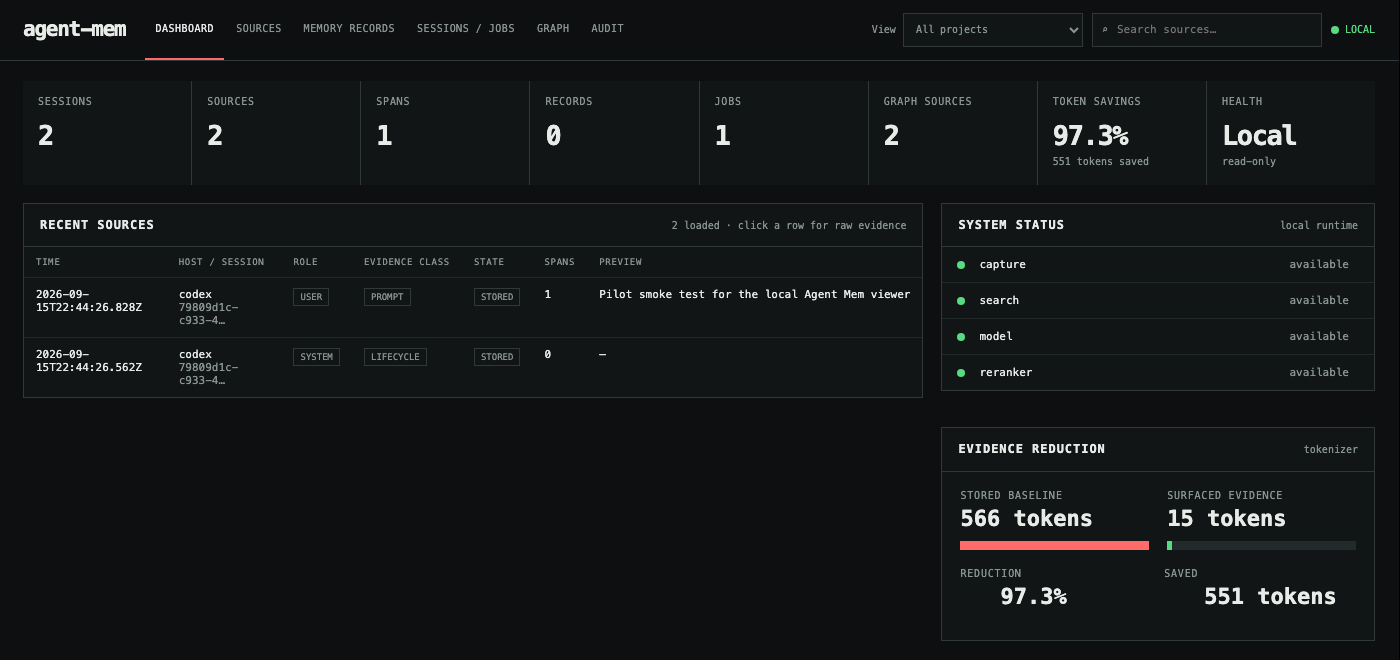
\includegraphics[width=0.98\linewidth,height=0.70\textheight,keepaspectratio]{agent-mem-ui-dashboard-compact-tight.png}
  \end{center}
\end{frame}

% 5 -------------------------------------------------------------------------
\begin{frame}{Persistence: What gets stored}
  \begin{center}
    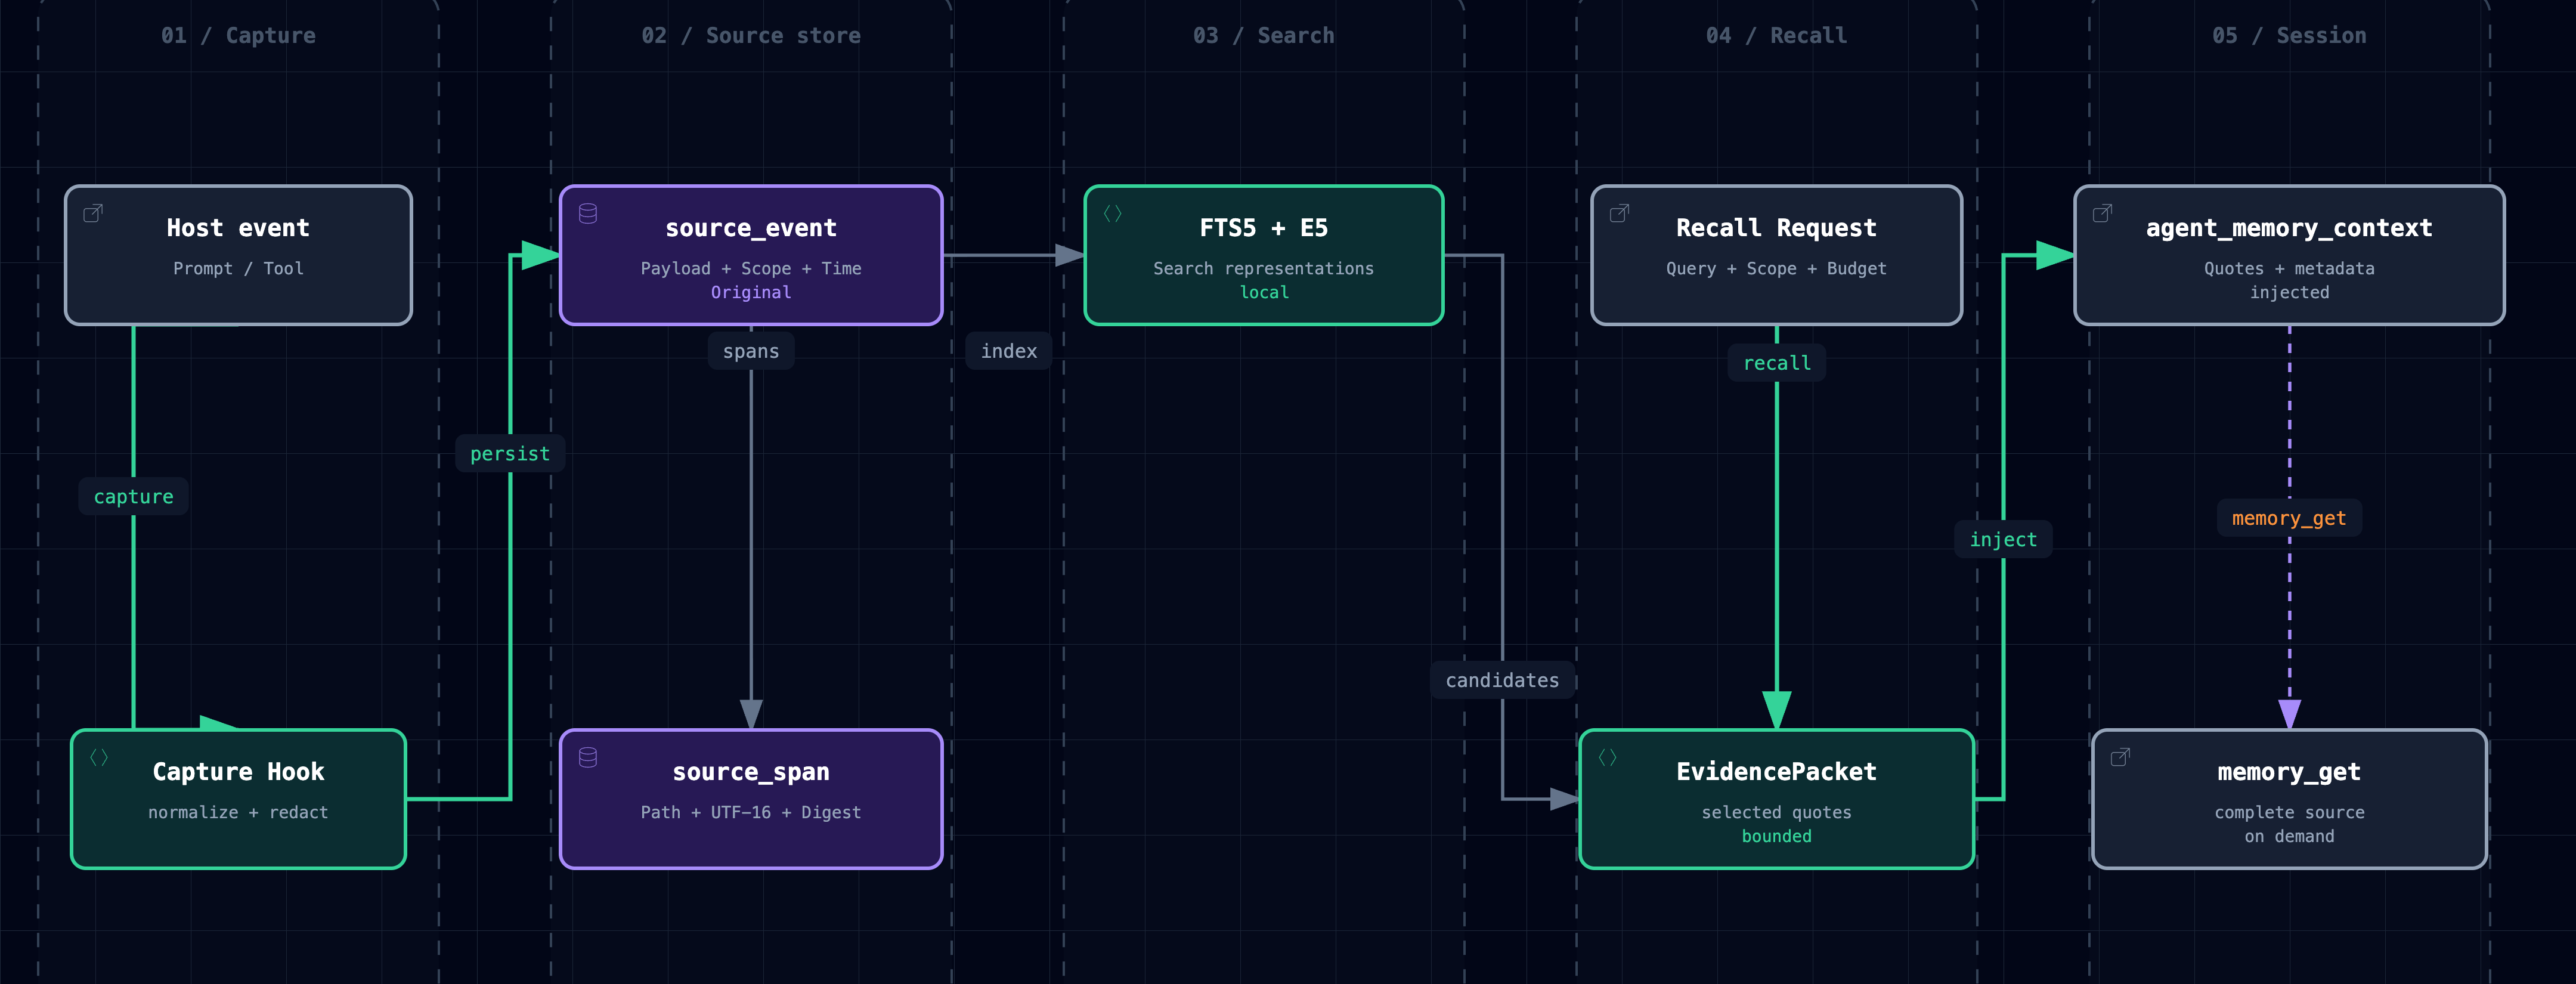
\includegraphics[width=0.98\linewidth,height=0.64\textheight,keepaspectratio]{agent-mem-storage-diagram-tight-en.png}
  \end{center}

  \vfill
  \begin{beamercolorbox}[wd=\dimexpr\linewidth-0.30cm\relax,sep=0.14cm,leftskip=0.15cm,rightskip=0.15cm]{block body}
    \footnotesize
    \amcode{source\_event}: payload + scope + time\qquad
    \amcode{source\_span}: path + UTF-16 offsets + digest\qquad
    \amcode{FTS5 / E5}: local search representations
  \end{beamercolorbox}
\end{frame}

% 6 -------------------------------------------------------------------------
\begin{frame}{Session context: What enters the session}
  \begin{center}
    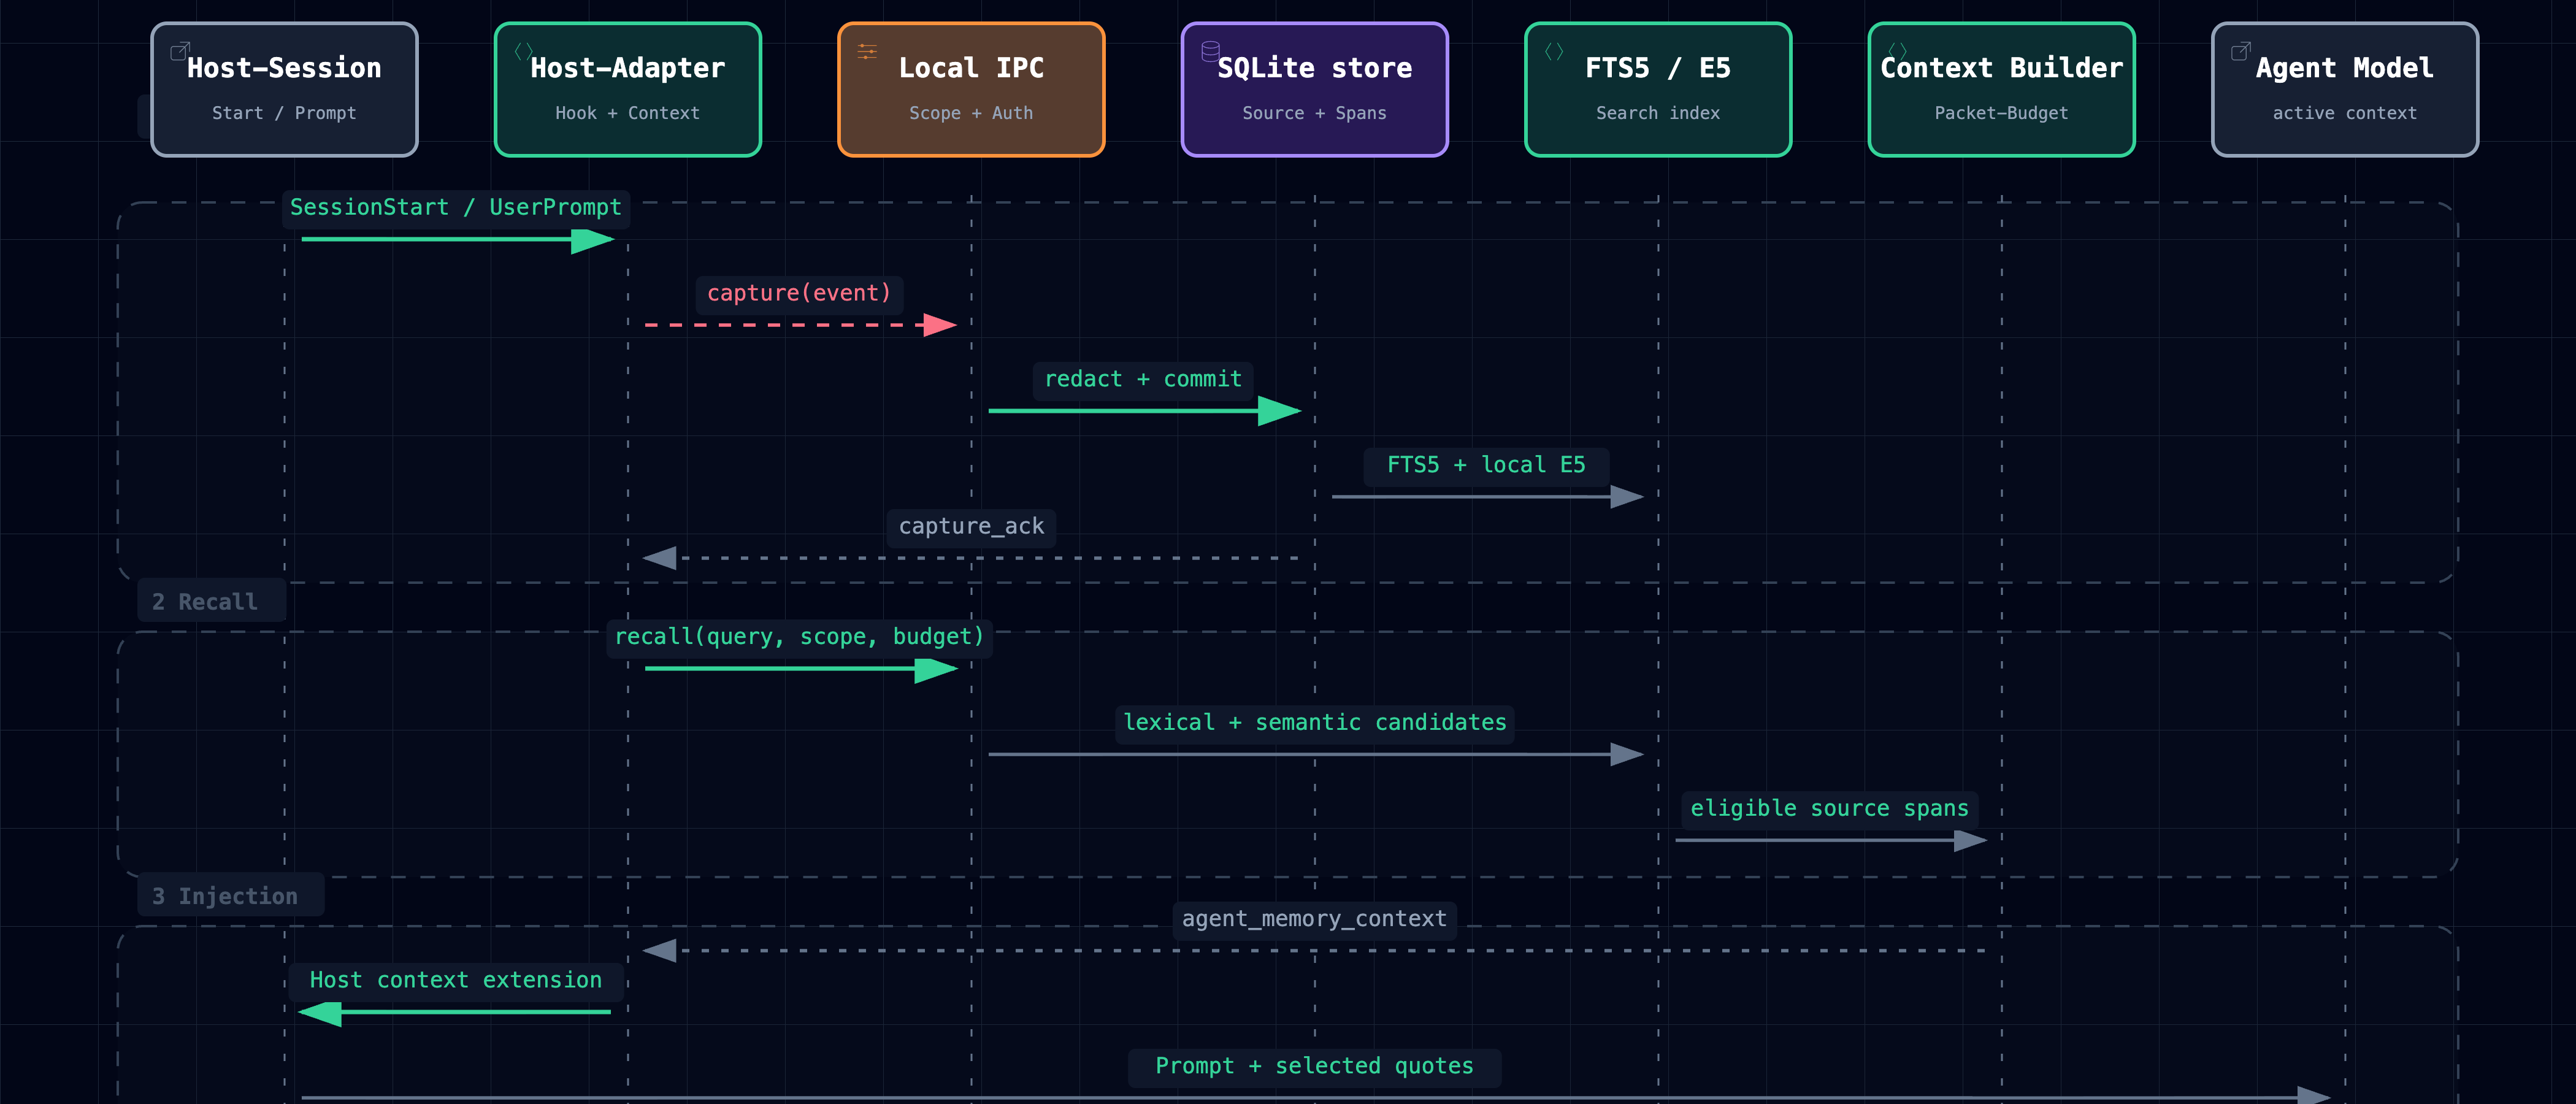
\includegraphics[width=0.98\linewidth,height=0.64\textheight,keepaspectratio]{agent-mem-session-sequence-tight-en.png}
  \end{center}

  \vfill
  \begin{beamercolorbox}[wd=\dimexpr\linewidth-0.30cm\relax,sep=0.14cm,leftskip=0.15cm,rightskip=0.15cm]{block body}
    \footnotesize
    \amcode{agent\_memory\_context}: injection ID + source IDs + scope + status + selected quotes.\quad
    The host receives a bounded packet.
  \end{beamercolorbox}
\end{frame}

% 7 -------------------------------------------------------------------------
\begin{frame}{Workflow in the Archify diagram}
  \begin{columns}[T,onlytextwidth]
    \column{0.31\textwidth}
      \amlabel{01 / CAPTURE}\\[0.16cm]

      {\Large\ttfamily\color{amViolet}Host event\par}

      \vspace{0.14cm}
      \small
      The capture hook cleans the event and writes \amcode{source\_event} and \amcode{source\_span}.

    \column{0.05\textwidth}
      \centering\textcolor{amLine}{\rule{0.45pt}{3.5cm}}

    \column{0.31\textwidth}
      \amlabel{02 / RECALL}\\[0.16cm]
      {\Large\ttfamily\color{amGood}Candidates\par}

      \vspace{0.14cm}
      \small
      FTS5 finds exact terms. E5 finds semantic variants. Scope and budget filter the selection.

    \column{0.05\textwidth}
      \centering\textcolor{amLine}{\rule{0.45pt}{3.5cm}}

    \column{0.28\textwidth}
      \amlabel{03 / INJECTION}\\[0.16cm]
      {\Large\ttfamily\color{amCoral}Session context\par}

      \vspace{0.14cm}
      \small
      \amcode{agent\_memory\_context} enters the session. \amcode{memory\_get} loads the source when needed.
  \end{columns}

  \vfill
  \begin{beamercolorbox}[wd=\dimexpr\linewidth-0.30cm\relax,sep=0.2cm,leftskip=0.15cm,rightskip=0.15cm]{block body}
    The diagram separates durable source data, candidate selection, and active session context.
  \end{beamercolorbox}
\end{frame}

% 8 -------------------------------------------------------------------------
\begin{frame}{Result and limits}
  \amlabel{CURRENT CORE}
  \vspace{0.20cm}

  {\fontsize{18}{22}\selectfont\ttfamily\color{amText}
    The store stays complete. The session stays bounded.\par}

  \vspace{0.25cm}
  \amrule
  \vspace{0.22cm}

  \begin{columns}[T,onlytextwidth]
    \column{0.47\textwidth}
    \amlabel{TODAY}\\[0.14cm]
      \normalsize
      \amcode{agent-mem} captures sources, searches locally, and returns only selected, source-grounded excerpts to the session.

    \column{0.06\textwidth}
      \centering\textcolor{amLine}{\rule{0.45pt}{2.5cm}}

    \column{0.47\textwidth}
    \amlabel{NEXT EXTENSION}\\[0.14cm]
      \normalsize
      Revisions, temporal models, and evaluation for stale or conflicting evidence.
  \end{columns}

  \vfill
  \begin{beamercolorbox}[wd=\dimexpr\linewidth-0.30cm\relax,sep=0.16cm,leftskip=0.15cm,rightskip=0.15cm]{block body}
    Every injected item points back to a stored source.
  \end{beamercolorbox}
\end{frame}

\end{document}
